% ---- Macros migrated from original lecture preamble ----
\providecommand\numberthis{\addtocounter{equation}{1}\tag{\theequation}}

\providecommand{\avg}{\mathrm{avg}}
\providecommand{\ID}{\mathrm{ID}}

\providecommand*\circled[1]{\tikz[baseline=(char.base)]{
            \node[shape=circle,draw,inner sep=2pt] (char) {#1};}}

\lecture{13}{May 20, 2025}{彭攀}{徐怡}{亚线性图算法：Sublinear Algorithms for Graphs}

当输入的规模过于庞大时，算法读取全部的输入需要花费大量的时间。因此，我们关心一类算法，只读取输入的极少一部分的信息，就能得到由理论保证的解——亚线性时间算法。
假设输入的规模是$N$，则亚线性时间算法的运行时间只需要$o(N)$。
亚线性时间算法的优良性质来自于对问题的近似以及随机性。特别地，本节课我们学习图数据结构上的亚线性时间算法。

\section{背景知识}
由于亚线性算法不能读取完整的输入，算法通过查询对输入进行访问。假设图的顶点集合是已知的，例如$V=\{1,2,\dots,n\}$，
但图的边集是未知的，需要查询。有以下三种标准的\textbf{查询模型}：
\begin{itemize}
    \item 邻接链表查询模型：对任意顶点$u$，可以查询其度数$\deg(u)$，以及它的邻居，可以通过存储一个邻接链表来实现。这个模型更适用于稀疏图。
    \item 邻接矩阵查询模型：对任意的点对$(u,v)$，在$O(1)$的时间内判断它们之间是否连边，可以通过存储一个邻接矩阵来实现。这个模型更适用于稠密图。
    \item 广义查询模型：既可以查询邻接链表，也可以查询邻接矩阵。即：可以查询任意顶点$u$的度数和邻居，也可以查询点对$(u,v)$是否连边。可以通过同时存储邻接链表和邻接矩阵来实现。
\end{itemize}

除此之外，有些算法会允许别的查询，比如边采样的查询，即在查询的时候返回一条均匀随机采样的边。
在接下来的笔记里，我们主要关注邻接链表查询模型。

除了查询模型，亚线性时间算法主要有以下几种\textbf{算法框架}：
\begin{itemize}
    \item 性质检测(Property Testing)：对于图的一些性质，如连通性、是否是平面图等，若图符合该性质，返回Yes；若图\textit{远离}该性质，返回No。
    \item 参数近似(Approximate Parameters)：近似图中的一些参数的\textit{数值}，如最小生成树的权重的值，最大匹配的大小的值等。
    \item 局部计算(Local Computation)：有时我们不只关心图的参数，还关注具体结构，如MST的结构。但光是输出MST就需要$\Omega(n)$的时间了。
    因此，在亚线性时间算法中，我们根据图的局部信息，揭示图的部分结构。例如对于任意一条边，返回其是否属于最小生成树，或者返回其是否属于最大匹配等。
\end{itemize}

前两种框架只输出一个数值，而第三种框架是在我们关心图的某种结构、但又不能花大量时间把结构完全输出时采取的。


\section{性质检测}
\textbf{目标：}通过查询模型对图进行访问，要求在尽可能少的查询次数下，判断图$G$是否具有性质$P$，或是\textit{远离}性质$P$。
例如：判断图的连通性，是否是二部图，能否进行3-染色，是否是平面图等。
如果图$G$具有性质$P$，以至少$\frac{2}{3}$的概率接受$G$；如果$G$远离性质$P$，以至少$\frac{2}{3}$的概率拒绝$G$。
对于既不满足$P$又不远离$P$的那部分图，我们不要求算法输出有保证的结果。

以检测图的连通性为例，思考如何辨别以下两种图：

\begin{figure}[!ht]
     \centering
     \begin{subfigure}[T]{0.48\textwidth}
        \centering
        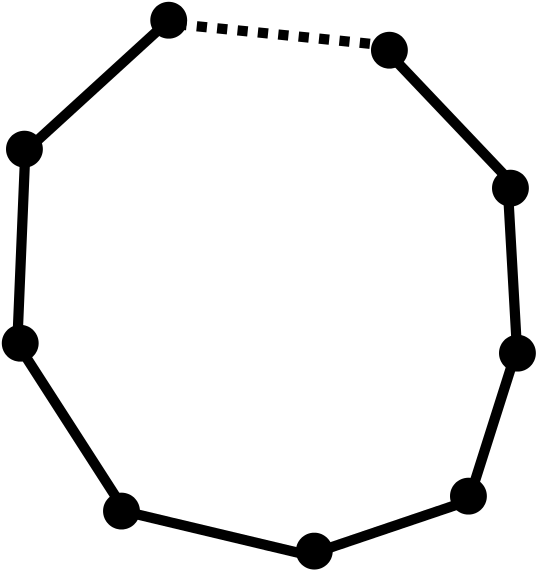
\includegraphics[width=.5\textwidth]{images/cycle.png}
        \caption*{\footnotesize{$G_1$：由$n$个点组成的环}}
     \end{subfigure}
     \hfill
     \begin{subfigure}[T]{0.48\textwidth}
         \centering
         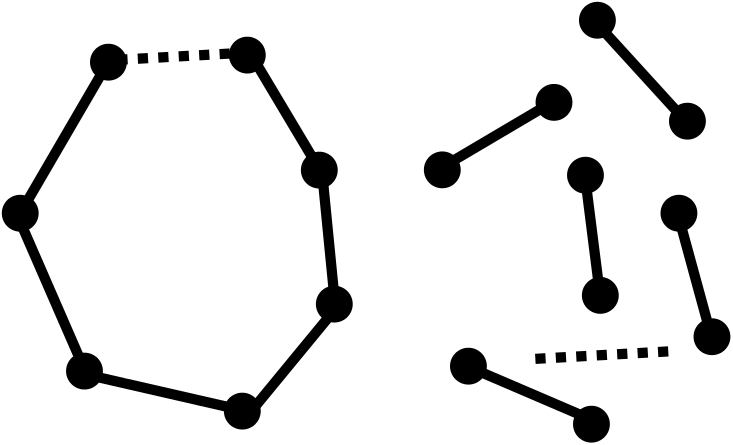
\includegraphics[width=.85\textwidth]{images/far.png}
        \caption*{\footnotesize{$G_2$：一个长为$\frac{n}{2}$的环$+ \frac{n}{4}$条互不相交的边}}
     \end{subfigure}
\end{figure}

为了区分$G_1$和$G_2$，可以采样常数个点（比如采样10个点），然后从采样的这些点出发，做两步广度优先搜索。
如果在搜索的过程中发现了孤立的边，说明是$G_2$，输出No（即不连通）。

\textbf{证明思路：}在$G_2$中，连着孤立边的点有$\frac{n}{4}\cdot 2=\frac{n}{2}$个，占总数的一半，均匀随机地采样10个点，采样的点全都没连到孤立边的概率是$(\frac{1}{2})^{10}$。
只要采样到孤立边对应的点，经过两步广度优先搜索，就一定能判断该图是$G_2$。
因此，以至少$1-\frac{1}{2^{10}}\ge\frac 23$的概率，采样10个点就能区分$G_1$和$G_2$。



如果要精确地判断一个任意的图是否连通，算法至少需要$\Omega(n+m)$次查询，例如，图中只有一个点是孤立的，其余所有点都连通，算法必须找到孤立点，则需要遍历所有的点。
因此，要设计亚线性时间的算法，我们允许算法对图的性质进行近似。



\subsection{检测连通性(度数受限图下的邻接链表模型)}
假设图$G$的最大度数是一个常数，记为$d$。远离性质$P$的形式化定义如下：
\begin{definition}
    如果需要对图$G$修改至少$\varepsilon dn$条边才能使得$G$满足性质$P$（修改边之后最大度数仍然是$d$），就称图$G$是$\varepsilon$-远离性质$P$的。
\end{definition}

例如，在\cref{fig:connectivity}中，左图是连通的，而右图更稀疏，需要添加很多条边才能连通，是\textit{远离}连通性的。

\begin{figure}[!ht]
     \centering
     \begin{subfigure}[T]{0.48\textwidth}
        \centering
        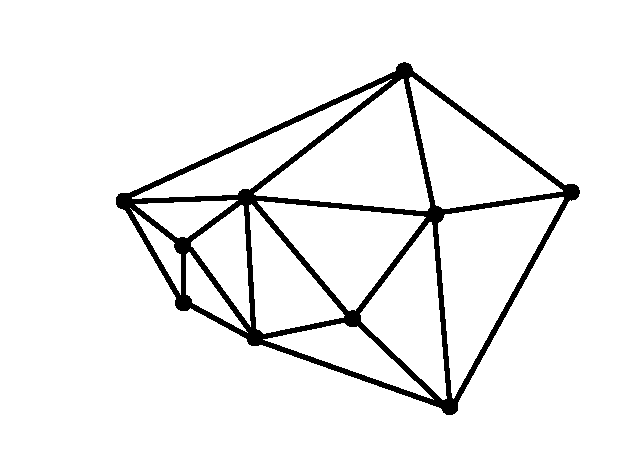
\includegraphics[height=4cm]{images/connected.eps}
	\caption*{连通图}
     \end{subfigure}
     \hfill
     \begin{subfigure}[T]{0.48\textwidth}
         \centering
         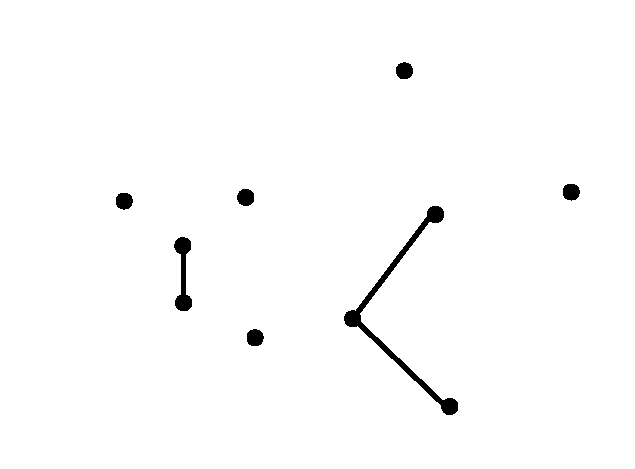
\includegraphics[height=4cm]{images/farconnected.eps}
	\caption*{远离连通性的图}
     \end{subfigure}
     \caption{图的连通性检测}
     \label{fig:connectivity}
\end{figure}

对于远离连通的图，我们观察到：如果一个图是远离连通的，
图中应该有大量较小的连通片（连通片的大小即该连通片包含的点的数量）。
因此我们通过采样一些点，再从这些点出发做广度优先搜索，就能把小的连通片挖掘出来，从而判断图的连通性。
这个观察可以形式化地表现为下面这个断言。
\begin{claim}[\cite{goldreich1997property}]\label{claim:smallCCs}
    如果图$G$是$\varepsilon$-远离连通性，则至少有$\frac{\varepsilon d n}{8}$个连通片的大小是$\le\frac{8}{\varepsilon d}$的。
\end{claim}

\begin{proof}
    记图$G$的连通片数量为$c$。当$G$不连通时，需要添加$c-1$条边才能使其连通（将所有连通片连起来）。
    由于$G$是$\varepsilon$-远离连通性，至少需要修改$\varepsilon dn$条边才能使$G$连通。
    因此，$c-1\ge\varepsilon dn$，即$c\ge\varepsilon dn$。

    记$G$中连通片大小超过$\frac{8}{\varepsilon d}$的数量为$c_1$，
    大小$\le\frac{8}{\varepsilon d}$的连通片的数量为$c_2$，则$c_1+c_2=c$。由于
    \[
    n=\text{$G$中的顶点数}=\sum_{\text{$G$中的连通片$S$}}|S|\ge\sum_{S:|S|>\frac{8}{\varepsilon d}}|S|\ge c_1\cdot\frac{8}{\varepsilon d}
    \]

    所以$c_1\le\frac{\varepsilon dn}{8}$，因此$c_2=c-c_1\ge \varepsilon dn-\frac{\varepsilon dn}{8}\ge\frac{\varepsilon dn}{8}$。
    该断言得证。
\end{proof}

基于以上观察，我们可以设计判断图的连通性的亚线性\textbf{算法}，\textsc{TestingConnectivity}：
\begin{enumerate}
    \item 重复$s=O(\frac{1}{\varepsilon d})$次迭代：
    \begin{enumerate}
        \item[1.1] 均匀随机地采样一个顶点$u$
        \item[1.2] 判断$u$所在的连通片的大小是否较小：
        \begin{enumerate}
            \item[1.2.1] 从$u$出发进行广度优先搜索。如果把$u$所在的连通片都访问完，
            或者已经访问了$t:=\Theta(\frac{1}{\varepsilon d})$个顶点，结束搜索。
            \item[1.2.2] 如果发现了一个大小$<t$的连通片，\textbf{拒绝}图$G$（即认为$G$远离连通性）
        \end{enumerate}
    \end{enumerate}
    \item \textbf{接受}图$G$（即认为$G$是连通的）
\end{enumerate}

\begin{algorithm}[h]
\caption{\textbf{连通性检测算法}}
	\label{alg-connectivity-test}
\begin{enumerate}
    \item \textbf{Input:} 一个整数 $ n \in \mathbb{Z}_{>0} $，$ \epsilon \in (0, 1) $，以及对图 $ G $ 上 $ n $ 个顶点的查询访问。
    \item \textbf{for} $ s := \Theta(1/(d \epsilon)) $ 次 \textbf{do}
    \begin{enumerate}
        \item 从 $ V $ 中随机均匀地抽样一个顶点 $ v $。
        \item 从 $ v $ 开始进行广度优先搜索（BFS），直到到达 $ 2/(d \epsilon) $ 个顶点，或者无法到达新的顶点为止。
        \item \textbf{if} 找到了一个（大小小于 $ n $ 的）连通分量 \textbf{then}
        \begin{enumerate}
            \item 拒绝。
        \end{enumerate}
        \item \textbf{end if}
    \end{enumerate}
    \item \textbf{end for}
    \item 接受。
\end{enumerate}
\end{algorithm}


\begin{theorem}[\cite{goldreich1997property}]
    算法\textsc{TestingConnectivity}能在$O(\frac{1}{\varepsilon^2d})$次查询内，检测图的连通性。
\end{theorem}

\begin{proof}
    \textbf{查询复杂度：}从每个被采样的点出发，广度优先搜索最多访问$\Theta(\frac{1}{\varepsilon d})$个点，
    最多有$\Theta(\frac{1}{\varepsilon d}\cdot d)=\Theta(\frac{1}{\varepsilon})$次查询。
    算法采样了$O(\frac{1}{\varepsilon d})$个点，因此总查询复杂度是$O(\frac{1}{\varepsilon d}\cdot\frac{1}{\varepsilon})=O(\frac{1}{\varepsilon^2 d})$。

    \textbf{正确性：}如果图$G$是连通的，算法\textsc{TestingConnectivity}不会发现大小$<t$的连通片，因此一定会接受$G$。
    如果$G$是$\varepsilon$-远离连通性，令$t=\frac{8}{\varepsilon d}$，则根据\cref{claim:smallCCs}，
    大小$<t$的连通片至少有$\frac{\varepsilon dn}{8}$个，占顶点总数的比例为$\frac{\varepsilon dn}{8}/n=\frac{\varepsilon d}{8}$。
    取$s=2/\frac{\varepsilon d}{8}=\frac{16}{\varepsilon d}$，
    则采样$s$个点均没有落在$<t$的连通片内的概率最多是
    \[
    \left(1-\frac{\varepsilon d}{8}\right)^s<e^{-\frac{\varepsilon d}{8}\cdot s}=e^{-2}<\frac{1}{3}
    \]

    因此，当$G$是$\varepsilon$-远离连通性时，以至少$\frac{2}{3}$的概率，采样的$s$个点中，至少存在一个点所在的连通片大小是$<t$，算法就会拒绝$G$。
\end{proof}

\subsection{检测二部性（稠密图上的邻接矩阵模型）}

在本节中，我们展示二分图性质是可用常数查询测试的。我们的算法同样简单明了：我们从顶点集 $ V $ 中抽样一个大小为常数的顶点集 $ S $，通过查询 $ S $ 中所有顶点对，得到诱导子图 $ G[S] $，然后检查该诱导子图 $ G[S] $ 是否为二分图。详见算法\Cref{alg-bipartite-test}。
\begin{algorithm}[h]
	\caption{\textbf{二部性检测算法}}
	\label{alg-bipartite-test}
	\begin{enumerate}
    \item \textbf{Input:} 一个整数 $ n \in \mathbb{Z}_{>0} $，$ \epsilon \in (0, 1) $，以及对图 $ G = (V, E) $ 上 $ n $ 个顶点的查询访问。
    \item 随机均匀地选择一个顶点集 $ S $，其中 $ |S| = \Theta(\epsilon^{-2} \log \epsilon^{-1}) $。
    \item 查询所有顶点对 $ (u, v) $，其中 $ u, v \in S $。
    \item \textbf{if} $ G[S] $ 是二分图 \textbf{then}
    \item \hspace{1em} 接受。
    \item \textbf{else}
    \item \hspace{1em} 拒绝。
    \item \textbf{end if}
\end{enumerate}
\end{algorithm}

\begin{theorem}
\Cref{alg-bipartite-test}以至少$2/3$的概率成功。
\end{theorem}
\begin{proof}
若 $G$ 是二分图，则其任意导出子图（包括 $G[S]$）也是二分图，因此算法会接受。

现在假设 $G$ 与任意二分图的距离至少为 $\epsilon$（即 $\epsilon$-远）。证明的主要思想如下：  
将采样集 $S$ 划分为两个不交集合 $T$ 与 $U$，其中  
$$
|T| = \frac{4}{\epsilon} \cdot \ln\!\left( \frac{\epsilon}{8/3} \right),
$$
集合 $U$ 由剩余的采样顶点组成。我们首先证明：以高概率，几乎所有顶点都至少有一个邻居在 $T$ 中。暂且假设这一条件成立。

考虑任意一个 $T$ 的二染色 $\chi : T \to \{\text{红}, \text{蓝}\}$。若要将 $\chi$ 扩展为整个图的合法二染色，一个必要条件是：红色顶点的邻居必须是蓝色，蓝色顶点的邻居必须是红色。这样，$T$ 的一个固定染色为 $V \setminus T$ 中的每个顶点施加了一个必要的颜色限制（若某顶点同时邻接红蓝两色顶点，则我们可视作它仅邻接蓝色顶点）。

据此，我们得到一个扩展染色 $\chi'$，它可能合法也可能不合法，但一定满足上述必要条件，且它为 $U$ 中的顶点确定了颜色。由于 $G$ 是 $\epsilon$-远离二分图的，因此在染色 $\chi'$ 下至少有 $\epsilon n^2$ 条单色边。

我们将 $U$ 划分为
$$
\epsilon^2 \cdot \big(|T| + \ln(6)\big)
$$
对（如果有剩余顶点则忽略）。任意一对顶点命中单色边的概率至少为 $\epsilon$，因此所有对都未命中单色边的概率至多为
$$
(1 - \epsilon)^{\epsilon^2 (|T| + \ln 6)} \le \frac{1}{6} \cdot 2^{-|T|}.
$$
因此：
$$
\Pr[\exists\ \text{$T \cup U$ 的合法二染色}] \le
\sum_{\chi \ \text{为}\ T\ \text{的二染色}} \Pr[U\ \text{对}\ \chi' \ \text{无单色边}]
\le 2^{|T|} \cdot \frac{1}{3} \cdot 2^{-|T|} = \frac{1}{3}.
$$

接下来考虑并非每个顶点都有邻居在 $T$ 的情形。定义
$$
\Gamma(T) = T \cup \{ v \in V \setminus T \mid \exists u \in T,\ (u,v) \in E \}.
$$

\begin{claim}
若 $|T| \ge \frac{4}{\epsilon} \ln\!\left( \frac{\epsilon}{8/3} \right)$，则以概率至少 $1 - \frac13$ 有
$$
\sum_{v \notin \Gamma(T)} \deg(v) \le \frac{\epsilon n^2}{2}.
$$
\end{claim}

\begin{proof}
对于度数至少 $\epsilon n/4$ 的顶点 $v$，有
$$
\Pr[v \notin \Gamma(T)] \le (1 - \epsilon/4)^{|T|} \le \frac{\epsilon}{8/3}.
$$
记 $X_v$ 为指示变量，表示事件 $v \notin \Gamma(T)$。则
$$
\mathbb{E}[X_v] \le \frac{\epsilon}{8/3}, \quad
\mathbb{E}\left[ \sum_{v \in V} X_v \right] \le \frac{\epsilon n}{8/3}.
$$
由 Markov 不等式可得
$$
\Pr\left[ \sum_{v \in V} X_v > \frac{\epsilon n}{4} \right] < \frac13.
$$
由于任意顶点度数 $\le n$，可得结论成立。
\end{proof}


假设 $T$ 是好的（即满足上述结论），并取 $T$ 的一个合法二染色 $\chi$。定义扩展染色 $\chi'$ 如下：
$$
\chi'(v) =
\begin{cases}
\chi(v), & v \in T, \\
1, & \exists u \in T, (u,v) \in E, \chi(u) = 2, \\
2, & \text{否则}.
\end{cases}
$$

\begin{claim}
若 $G$ 是 $\epsilon$-远离二分图，且 $\sum_{v \notin \Gamma(T)} \deg(v) \le \frac{\epsilon n^2}{2}$，则在 $\Gamma(T)$ 中由 $\chi'$ 诱导的单色边数超过 $\frac{\epsilon n^2}{2}$。
\end{claim}

\begin{proof}
由于 $G$ 是 $\epsilon$-远离二分图，任何染色 $\chi'$ 都至少有 $\epsilon n^2$ 条单色边。其中至多 $\frac{\epsilon n^2}{2}$ 条与 $V \setminus \Gamma(T)$ 相邻，因此 $\Gamma(T)$ 中的单色边数超过 $\frac{\epsilon n^2}{2}$。
\end{proof}

最后，将 $U$ 划分为
$$
\frac{2}{\epsilon} \cdot \left(|T| + \ln 6\right)
$$
对。由上述引理，每对顶点命中单色边的概率至少为 $\epsilon/2$，因此无对命中单色边的概率至多
$$
(1 - \epsilon/2)^{\epsilon^2 (|T| + \ln 6)} \le \frac{1}{6} \cdot 2^{-|T|}.
$$
综合各项概率估计可知，算法接受的概率至多 $1/3$，因此拒绝的概率至少为 $2/3$。
\end{proof}

\section{参数近似}
\textbf{目标：}通过查询模型对图进行访问，要求在尽可能少的查询次数下，比较好地近似图中的一些参数。例如：最小生成树的权重的值，边的数量，最大匹配的大小，给定子图的数量等。

\subsection{估算最小生成树的权重}
在本小节中，我们研究近似最小生成树的权重。即：在图$G=(V,E)$中找到一棵树$T\subseteq E$，
使得树的权重$w(T)=\sum_{(u,v)\in T}w(u,v)$最小。最小的权重对应的树记为$T^*$，其权重记为$w(G)=w(T^*)$。
注意到，如果精确地计算最小生成树或者其权重，需要线性的时间，但我们可以在亚线性时间内对其权重进行近似。

\subsubsection{最小生成树权重的公式}

\begin{definition}
    记$G^{(\ell)}$表示$G$的子图，$G^{(\ell)}$的顶点集合与$G$相同，
    边集包含$G$中所有权重$\le\ell$的边。记$G^{(\ell)}$中连通片的数量为$c^{(\ell)}$。
\end{definition}

基于上述定义，我们有以下观察：

\begin{claim}\label{claim:MST-CC}
    记$n=|V|$为图$G$的顶点数，$W$表示$G$的最大权重。则$G$中最小生成树的权重满足：$w(G)=n-W+\sum_{i=1}^{W-1}c^{(i)}$。
\end{claim}
\begin{proof}
    记MST中权重为$i$的边的数量为$\alpha_i$，根据Kruskal算法，不同的MST中，$\alpha_i$的值是一样的。
    观察到：
    \begin{itemize}
        \item $\sum_{i=1}^W \alpha_i=n-1$，因为最小生成树上一共有$n-1$条边
        \item 对于任意的$\ell\in[W]$，有$\sum_{i>l}\alpha_i=c^{(\ell)}-1$，因为要想把$G^{(\ell)}$中的所有连通片连起来，
        需要用到$c^{(\ell)-1}$条边，而这些边的权重都$>\ell$，且使用最小生成树上的边就足够把这些连通片连起来了（因为最小生成树是连通的）
        \item $c^{(0)}=n$，因为已经假设图$G$的边权属于$\{1,\dots,W\}$，没有一条边的权重是0，
        因此$G^{(0)}$中没有一条边，每个顶点都是孤立点
    \end{itemize}

    因此，最小生成树的权重可以写成：
    \begin{align*}
        w(G)=&\sum_{i=1}^W i\cdot\alpha_i\\
        &=\sum_{j=1}^W(\sum_{i=j}^W \alpha_i)\\
        &=\sum_{j=1}^W (c^{(j-1)}-1) \tag{利用$\sum_{i>\ell}\alpha_i=c^{(\ell)}-1$}\\
        &=n-W+\sum_{j=1}^{W-1}c^{(j)}
    \end{align*}
\end{proof}

\subsubsection{估算连通片的数量}
有了\cref{claim:MST-CC}，我们就只需要估算$c^{(\ell)}$，即每个子图$G^{(\ell)}$的连通片的数量。

对顶点$u$，记$n(u)$表示$u$所在的连通片中顶点的数量。
对任意连通片$A$，观察到：$\sum_{u\in A}\frac{1}{n(u)}=\sum_{u\in A}\frac{1}{|A|}=1$。
进一步，记图$G$的全体连通片的集合为$\cC$，则有：
$\sum_{v\in V}\frac{1}{n(v)}=\sum_{A\in\cC}\sum_{u\in A}\frac{1}{n(u)}=\sum_{A\in\cC}1=|\cC|$，即图中连通片的数量。

因此，如果对每个顶点$v$，$n(v)$的值是已知的，
我们只需要进行简单的操作即可估算连通片的数量：
\begin{enumerate}
    \item 将求和$sum$初始化为0
    \item 重复$s$次迭代：
    \begin{enumerate}
        \item[2.1] 均匀随机地采样一个点$v\in V$
        \item[2.2] 计算$sum\leftarrow sum+\frac{1}{n(v)}$
    \end{enumerate}
    \item 输出$\tilde{c}=n\cdot\frac{sum}{s}$
\end{enumerate}

当然，实际情况中，$n(v)$是未知的，因此我们考虑估算$n(v)$的值。
参考算法\textsc{TestConnectivity}，我们得到一个估算连通片数量的\textbf{算法}$\cA$：
\begin{enumerate}
    \item 将求和$sum$初始化为0
    \item 重复$s=O(1/\varepsilon^3)$次迭代：
    \begin{enumerate}
        \item[2.1] 均匀随机地采样一个点$v\in V$
        \item[2.2] 从$v$出发做广度优先搜索，如果在遍历完整个连通片之前访问了超过
        $\frac{2}{\varepsilon}$个顶点，令$\tilde{n}(v)=\frac{2}{\varepsilon}$；
        
        否则，如果遍历完整个连通片时访问的点数$\le\frac{2}{\varepsilon}$，
        令$\tilde{n}(v)=n(v)$，即访问的点数
        \item[2.3] 计算$sum\leftarrow sum+\frac{1}{\tilde{n}(v)}$
    \end{enumerate}
    \item 输出$\tilde{c}=n\cdot\frac{sum}{s}$
\end{enumerate}

\begin{lemma}\label{lem:appncc}
    对于图$G$，记其连通片的数量为$c$。上述算法$\cA$
    输出的估计值$\tilde{c}$，以至少$\frac{2}{3}$的概率满足$|\tilde{c}-c|\le\varepsilon n$。
    算法$\cA$的运行时间为$O(\frac{d}{\varepsilon^4})$
\end{lemma}
\begin{proof}
    \textbf{运行时间：}对于每个采样的顶点，从它出发探索的点数最多为$\frac{2}{\varepsilon}$，
    由于顶点度数最大是$d$，因此广度优先搜索的时间是$O(\frac{d}{\varepsilon})$。
    因为采样了$O(1/\varepsilon^3)$个顶点，所以总的运行时间为$O(\frac{d}{\varepsilon}/\varepsilon^3)=O(\frac{d}{\varepsilon^4})$。

    \textbf{正确性：}记
    $\hat{n}(u)=\min\{n_u,\frac{2}{\varepsilon}\}$，
    $\hat{c}:=\sum_{u\in V}\frac{1}{\hat{n}(u)}$。
    则：对于任意的顶点$u$，$|\frac{1}{\hat{n}(u)}-\frac{1}{n(u)}|\le\frac{\varepsilon}{2}$。
    因为当$n_u<\frac{2}{\varepsilon}$时，$\hat{n}(u)=n(u)$，此时$\frac{1}{\hat{n}(u)}-\frac{1}{{n}(u)}=0$；
    而当$n_u\ge\frac{2}{\varepsilon}$时，$0<\frac{1}{{n}(u)}\le\frac{1}{\hat{n}(u)}=\frac{\varepsilon}{2}$，
    所以$\frac{1}{\hat{n}(u)}-\frac{1}{{n}(u)}\le\frac{\varepsilon}{2}$。

    因此，有$|\hat{c}-c|=|\sum_{u\in V}\frac{1}{\hat{n}(u)}-\frac{1}{n(u)}|\le\sum_{u\in V}|\frac{1}{\hat{n}(u)}-\frac{1}{{n}(u)}|
    \le\sum_{u\in V}\frac{\varepsilon}{2}=\frac{\varepsilon n}{2}$。

    此外，由于$1\le\hat{n}(u)\le\frac{2}{\varepsilon}$，对任意的$u$，有$\frac{\varepsilon}{2}\le\frac{1}{\hat{n}(u)}\le1$，
    因此$\frac{\varepsilon n}{2}\le\hat{c}\le n$。

    对于第$i$个采样的点，记估计值$\frac{1}{\tilde{n}(u)}$为$X_i\in[0,1]$，计算它的期望：
    $\E[X_i]=\frac{1}{n}\sum_{u\in V}\frac{1}{\hat{n}(u)}=\frac{\hat{c}}{n}$。

    由于$\frac{s}{n}\tilde{c}=\sum_{i=1}^s X_i$，其期望为
    $\E[\sum_{i=1}^s X_i]=s\cdot \E[X_1]=\frac{s\hat{c}}{n}$。
    记$X=\sum_{i=1}^s X_i$，
    根据Chernoff-Hoeffding Bound（见笔记\textit{Notes Lec1 概率论回顾}），有
    \begin{align*}
        \Pr[|\tilde{c}-\hat{c}|\ge\frac{\varepsilon \hat{c}}{2}]&=\Pr[|\frac{s}{n}\tilde{c}-\frac{s}{n}\hat{c}|\ge\frac{\varepsilon}{2}\cdot\frac{s\hat{c}}{n}]\\
        &=\Pr[|X-\E[X]|\ge\frac{\varepsilon}{2}\E[X]]\\
        &\le 2\exp(-\frac{\E[X]\cdot\varepsilon^2/2^2}{3})\\
        &=2\exp(-\frac{s\hat{c}\varepsilon^2}{12n}) \tag{代入$\E[X]$}\\
        &\le2\exp(-O(\frac{1}{\varepsilon^3})\cdot\frac{\varepsilon n}{2}\cdot\frac{\varepsilon^2}{12n}) \tag{由于$s=O(1/\varepsilon^3)$且$\hat{c}\ge\frac{\varepsilon n}{2}$}\\
        &\le\frac{1}{3} \tag{通过选取$s=b/\varepsilon^3$中的常数$b$可以实现}
    \end{align*}

    因此，以至少$\frac{2}{3}$的概率，$|\tilde{c}-c|\le|\tilde{c}-\hat{c}|+|\hat{c}-c|\le\frac{\varepsilon\hat{c}}{2}+\frac{\varepsilon n}{2}\le \varepsilon n$。
\end{proof}

\subsubsection{估算最小生成树权重的算法}

根据算法$\cA$，设计估算最小生成树权重的\textbf{算法}$\cB$：
令$\varepsilon'=\frac{\varepsilon}{W}$，再使用median trick增强算法的成功概率，对每个子图$G^{(i)}$调用算法$\cA$得到$\tilde{c}^{(i)}$。
输出$\tilde{w}(G)=n-W+\sum_{i=1}^{W-1}\tilde{c}^{(i)}$。

\begin{theorem}\label{thm:appmst}
    图$G$有$n$个顶点，假设图中每条边的权重都是区间$[1,W]$内的整数，
    则存在一个算法输出估计值$\tilde{w}(G)$，以至少$\frac{2}{3}$的概率满足
    \[
    (1-\varepsilon)\cdot w(G)\le \tilde{w}(G)\le(1+\varepsilon)\cdot w(G)
    \]

    该算法的运行时间为$\tilde{O}(d\cdot W^5/\varepsilon^5)$。
\end{theorem}
\begin{proof}
    根据\cref{lem:appncc}，算法$\cB$得到的任意一个$\tilde{c}^{(i)}$以至少$1-\frac{1}{\poly(W)}$的概率满足$|\tilde{c}^{(i)}-c^{(i)}|\le\frac{\varepsilon n}{W}$。
    因此，利用union bound，对\textit{所有的}$i\in[W]$，该不等式都满足的概率是$1-\frac{1}{\poly(W)}$。下面假设这个事件发生。

    得到$\tilde{w}(G)$的运行时间为
    $W\cdot\tilde{O}(\frac{d}{(\varepsilon/W)^4})=\tilde{O}(\frac{W^5d}{\varepsilon^4})$。
    其理论保证为
    \begin{align*}
        |w(G)-\tilde{w}(G)|&=\left|\left(n-W+\sum_{i=1}^{W-1}{c}^{(i)}\right)-\left(n-W+\sum_{i=1}^{W-1}\tilde{c}^{(i)}\right)\right| \tag{根据\cref{claim:MST-CC}}\\
        &\le\sum_{i=1}^{W-1}|\tilde{c}^{(i)}-c^{(i)}| \\
        &\le(W-1)\frac{\varepsilon n}{W} \tag{根据$\tilde{c}^{(i)}$的理论保证}\\
        &<\varepsilon n\\
        &\le 2\varepsilon\cdot w(G) \tag{由于$c^{(i)}\ge 1$，$w(G)\ge n-W+W-1\ge\frac{n}{2}$，当$n\ge2$时}
    \end{align*}
\end{proof}

\subsection{估算图的平均度数}
\problem 对于一个\textbf{连通}的图$G=(V,E)$，其顶点集合为$V=[n]:=\{1,\dots,n\}$。
图中一个点$v$的度数，是和它相连的边数，记为$\deg(v)$。
对图的访问可以是仅允许查询任意顶点的度数，也可以包含查询顶点的邻居。
目标是在亚线性时间内估算图的平均度数，即估算$d_{\avg}=\frac{1}{n}\sum_{v\in V}\deg(v)$。

\subsubsection{查询图的度数}
如果只允许查询图中顶点的度数（不允许查询顶点的邻边），这个问题是很难的。

考虑一个星状图$G_1$，即一个中心点连着其他所有顶点，除此之外图中没有别的边。
在这个图里，只有一个顶点的度数是$n-1$，其余顶点的度数都是$1$，
平均度数为$d_{\avg}=\frac{(n-1)\cdot1+1\cdot(n-1)}{n}\approx2$。
要做到2-近似，就一定要访问中心点，否则得到的平均度数是1（2-近似指，算法输出的估算值$R$满足$d_{\avg}\le R\le2d_{\avg}$）。

更进一步，考虑图$G_2$，其中有100个顶点的度数是$n-1$，其余顶点的度数都是1，
平均度数为$d_{\avg}=\frac{(n-100)\cdot1+100\cdot(n-1)}{n}\approx 101$，
那要想做到比100更好的近似比，就需要找到这100个特殊的顶点，需要$\Omega(n)$次查询。
100也可以换成别的常数，这样看来似乎在亚线性时间下，常数近似都做不到。
但$G_2$这样的图是不存在的，因为顶点的度数需要符合图数据结构的规则。

事实上，存在一个亚线性时间的\textbf{算法}\textsc{AvgDeg-V1}，可以做到$(2+\varepsilon)$-近似：
\begin{enumerate}
    \item 调用子程序\textsc{AvgNibble} $t:=\frac{8}{\varepsilon}$次，
    得到估算值$d_{S_1},\dots,d_{S_t}$
    \item 输出这些估算值中的最小值，即输出$R:=\min_{i=1}^t d_{S_i}$
\end{enumerate}

子程序\textsc{AvgNibble}的描述如下：
\begin{enumerate}
    \item 给定某个足够大的常数$\beta>0$，
    采样$s=\frac{\beta\sqrt{n}}{\varepsilon^3}$个点，采样的顶点集合记为$S$
    \item 输出采样的点的平均度数，即输出$d_S:=\frac{\sum_{i\in S}\deg(i)}{s}$
\end{enumerate}


\begin{theorem}\label{thm:avgdeg-v1}
    令$0<\varepsilon<\frac{1}{3}$为一个常数。
    假设算法只允许查询顶点的度数，则\textsc{AvgDeg-V1}算法输出的$R$
    以至少$\frac{3}{4}$的概率满足
    $(\frac{1}{2}-\varepsilon)d_{\avg}\le R\le(1+\varepsilon)d_{\avg}$，
    且运行时间为$O(\sqrt{n}/\varepsilon^4)$。
\end{theorem}

注意到，根据\cref{thm:avgdeg-v1}，有$d_{\avg}\le\frac{1}{1/2-\varepsilon}R\le\frac{1+\varepsilon}{1/2-\varepsilon}d_\avg$，
其中由于$\frac{1}{1-2\varepsilon}\le 1+3\varepsilon$，有
$\frac{1+\varepsilon}{1/2-\varepsilon}\le(2+2\varepsilon)(1+3\varepsilon)=2+O(\varepsilon)$。
令$R'=\frac{1}{1/2-\varepsilon}R$，则$R'$的近似比为$2+\varepsilon$。

为了证明\cref{thm:avgdeg-v1}，需要先证两个引理。

\begin{lemma}\label{lem:nibble-A}
    以至少$1-\frac{1}{1+\varepsilon}\ge\frac{\varepsilon}{2}$的概率，
    算法\textsc{AvgNibble}输出的$d_S$满足$d_S\le(1+\varepsilon)\cdot d_\avg$。
\end{lemma}
\begin{proof}
    令$X_i$表示第$i$个采样的点的度数，由于是均匀随机采样，
    有$\Pr[\text{第$i$个被采样到的顶点为}j]=\Pr[X_i=\deg(j)]=\frac{1}{n}$，。
    因此，
    \[
    \E[X_i]=\sum_{j=1}^n\deg(j)\Pr[X_i=\deg(j)]=\sum_{j=1}^n\deg(j)\cdot\frac{1}{n}=d_\avg
    \]

    由于$d_S=\frac{\sum_{i\in S}\deg(i)}{s}$，
    有$\E[d_S]=\E[\frac{1}{s}\sum_{i=1}^sX_i]=d_\avg$。
    根据Markov不等式，
    \[
    \Pr[d_S>(1+\varepsilon)d_\avg]\le\frac{\E[d_S]}{(1+\varepsilon)d_\avg}=\frac{1}{1+\varepsilon}
    \]
\end{proof}

\begin{lemma}\label{lem:nibble-B}
    以至少$1-\frac{\varepsilon}{64}$的概率，
    算法\textsc{AvgNibble}输出的$d_S$满足$d_S\ge(\frac{1}{2}-\varepsilon)\cdot d_\avg$。
\end{lemma}
\begin{proof}
    对于图$G=(V,E)$，定义$H$为度数最高的$\sqrt{\frac{\varepsilon}{2}n}$个顶点的集合，
    $L=V\setminus H$。

    首先，由于$\sum_{i=1}^n\deg(i)=2|E|$，则$L$和$H$之间的边满足
    $|E(L,H)|\le|E|\le\frac{1}{2}\sum_{i=1}^n\deg(i)$。

    其次，由于$H$中只有$\sqrt{\frac{\varepsilon}{2}n}$个顶点，所以
    $2|E(H)|\le|V(H)|^2=\frac{\varepsilon n}{2}$。

    此外，由于图$G$是连通的，至少有$n-1$条边，所以$\sum_{i=1}^n\deg(i)=2|E|\ge2(n-1)$。
    因此，有
    \[
    2|E(H)|\le\frac{\varepsilon}{2}n\le\frac{\varepsilon}{2}2(n-1)
    \le\frac{\varepsilon}{2}\cdot\sum_{i=1}^n\deg(i)
    \]

    $L$中的点的度数之和满足$\sum_{i\in L}\deg(i)=\sum_{i=1}^n\deg(i)-|E(L,H)|-2|E(H)|$。
    记$L$中顶点的平均度数为$d_L$，则有
    $d_L=\frac{\sum_{i\in L}\deg(i)}{|L|}\ge\frac{(\frac{1}{2}-\frac{1}{2}\varepsilon)\sum_{i=1}^n\deg(i)}{n}=(\frac{1}{2}-\frac{1}{2}\varepsilon)d_\avg$。

    由于这个引理在求$d_S$的下界，我们可以假设所有采样到的顶点都来自$L$。
    定义$D_H$为$H$中最小的度数，$X_i$为第$i$个被采样到的顶点的度数。
    则$\E[X_i]\ge d_L=\frac{\sum_{i\in L}\deg(i)}{|L|}\ge(\frac{1}{2}-\frac{1}{2}\varepsilon)d_\avg$。
    
    由于$d_S=\frac{\sum_{i=1}^sX_i}{s}$，则$E[d_S]=\frac{1}{s}\E[\sum_{i=1}^sX_i]\ge(\frac{1}{2}-\frac{1}{2}\varepsilon)d_\avg$。
    等价地，有$(\frac{1}{2}-\varepsilon)d_\avg\le\frac{\frac{1}{2}-\varepsilon}{\frac{1}{2}-\frac{1}{2}\varepsilon}\E[d_S]\le(1-\varepsilon)\E[d_S]$。

    另一方面，对于平均度数，有$d_\avg=\frac{1}{n}\sum_{i=1}^n\deg(i)\ge\frac{\sum_{i\in H}\deg(i)}{n}\ge\frac{D_H\cdot|H|}{n}$，
    因此$\E[d_S]\ge\frac{(\frac{1}{2}-\frac{1}{2}\varepsilon)D_H\cdot|H|}{n}$，
    且$\E[\sum_{i=1}^sX_i]\ge\frac{(\frac{1}{2}-\frac{1}{2}\varepsilon)D_H\cdot|H|\cdot s}{n}$。
    根据Chernoff Bound，有
    \begin{align*}
        \Pr[d_S\le(\frac{1}{2}-\varepsilon)d_\avg]&\le\Pr[d_S\le(1-\varepsilon)\E[d_S]]\\
        &=\Pr[\frac{1}{s}\sum_{i=1}^sX_i\le(1-\varepsilon)\frac{1}{s}\E[\sum_{i=1}^sX_i]]\\
        &=\Pr[\frac{1}{D_H}\sum_{i=1}^sX_i\le(1-\varepsilon)\frac{1}{D_H}\E[\sum_{i=1}^sX_i]]\\
        &\le2\exp(\frac{-\E[\sum_{i=1}^sX_i]\cdot\varepsilon^2}{3\cdot D_H}) \tag{假设采样的点都来自$L$，有$0\le\frac{X_i}{D_H}\le1$}\\
        &\le2\exp(\frac{-s\cdot|H|}{n}\cdot(\frac{1}{2}-\frac{1}{2}\varepsilon)\cdot\frac{\varepsilon^2}{3})\\
        &\le2\exp(\frac{-s\cdot \varepsilon^{2.5}}{100\sqrt{n}})
    \end{align*}

    因此，令$s=\frac{200\sqrt{n}}{\varepsilon^3}$，即有
    $\Pr[d_S\le(\frac{1}{2}-\varepsilon)d_\avg]\le\frac{\varepsilon}{64}$。
\end{proof}

有了\cref{lem:nibble-A}和\cref{lem:nibble-B}，我们就能证得\cref{thm:avgdeg-v1}。

\begin{proof}[\cref{thm:avgdeg-v1}的证明]
    首先，根据\cref{lem:nibble-B}，以及$(1-\frac{1}{x+1})^x\ge\frac{1}{e}$，有：
    \[
    \Pr[R\ge(\frac{1}{2}-\varepsilon)]=\Pr[\forall i\in[t],d_{S_i}\ge(\frac12-\varepsilon)d_\avg]
    \ge(1-\frac{\varepsilon}{64})^{\frac{8}{\varepsilon}}>\frac{7}{8}
    \]

    其次，根据\cref{lem:nibble-A}，以及$(1-\frac{1}{x})^x\le\frac{1}{e}$，有：
    \begin{align*}
        \Pr[R\le(1+\varepsilon)d_\avg]&=\Pr[\exists i\in[t], d_{S_i}\le(1+\varepsilon)d_\avg]\\
        &=1-\Pr[\forall i\in[t], d_{S_i}>(1+\varepsilon)d_\avg]\\
        &>1-(1-\frac{\varepsilon}{2})^t\\
        &>1-\frac{1}{16}
        \end{align*}
\end{proof}


\subsubsection{查询图的度数和边}
如果算法同时可以访问顶点的度数和邻边，估算平均度数就会容易很多。
在之前的$G_1$的例子中，只能访问顶点度数的算法必须要发现度数为$n-1$的顶点，
才能实现2-近似。但如果算法能访问顶点的邻边，就能很容易地发现度数较高的顶点。

首先先假设一个更简单的情况：假设图$G$是一个几乎正则的图，图中顶点的度数相差不大，
每个顶点的度数都属于区间$[d,10d]$，没有奇异点（即少数点的度数特别大，达到$O(n)$的级别）。
这样的话，算法可以采样一些顶点，计算它们的平均度数。\textbf{算法}描述如下：

\begin{enumerate}
    \item 令$k=\frac{50}{\varepsilon^2}\cdot\ln(\frac{2}{\delta})$，
    \item 对于$i=1,\dots,k$：
    \begin{enumerate}
        \item[2.1] 均匀随机地采样一个顶点，记为$v_i$
        \item[2.2] 令$X_i=\deg(v_i)$
    \end{enumerate}
    \item 输出$\tilde{d}=\frac{1}{k}\sum_{i=1}^kX_i$
\end{enumerate}

\begin{claim}
    上述算法输出的估算值$\tilde{d}$满足$\E[\tilde{d}]=d_\avg$。
\end{claim}

\begin{claim}
    上述算法输出的估算值$\tilde{d}$满足$\Pr[|\tilde{d}-d_\avg|\le\varepsilon d_\avg]\ge1-\delta$，
    且运行时间为$O(\frac{1}{\varepsilon^2}\log\frac{1}{\delta})$。
\end{claim}

在几乎正则的图里，顶点度数的方差很小，因此采样法很有效；
但在一般的图里，有些顶点度数很高，使得方差很大。
如果仍然用最简单的采样法来估计，需要的运行时间是$O(\frac{n}{\varepsilon^2}\cdot\log\frac{1}{\delta})$。

\idea 我们可以考虑减小度数高的顶点带来的方差。由于图的边数是有限的（$|E|=m$），度数很高的顶点不会太多，
我们可以通过引入$\deg^+(v)$，把每条边分配给度数较低的点，从而减小高度数顶点的影响。

具体来说，先定义一个偏序关系$\prec$：如果$\deg(u)<\deg(v)$，或者$\deg(u)=\deg(v)$且$\ID(u)<\ID(v)$，
则称$u\prec v$。
其中，$\ID(v)$表示顶点$v$在集合$V$中的字典序，是输入给定的顺序。
接着，定义$\deg^+(u):=\#\{v\in N(u)|u\prec v\}$，即$u$的邻居中满足$u\prec v$的顶点数。
那么：$\sum_{v\in V}\deg^+(v)=m=\frac{n}{2}\cdot d_\avg$。

尽管一般图中的$\deg(v)$的确会非常大，从而带来很大的方差；
但我们将证明，$\deg^+(v)$对每个顶点$v$来说都是有界的，因此方差更小，
估算$\deg^+(v)$能有更好的理论保证。

\begin{definition}
    定义$H\subset V$是在偏序关系$\prec$下前$\sqrt{2m}$大的顶点集合。
    定义$L:=V\setminus H$。
\end{definition}

\begin{claim}\label{claim:LH-bound}
    对任意顶点$v\in H$，有$\deg^+(v)\le\sqrt{2m}$。

    对任意顶点$v\in L$，有$\deg(v)\le\sqrt{2m}$。
\end{claim}
\begin{proof}
    对于任意$H$中的顶点$v$，$\deg^+(v)$只包含在偏序关系$\prec$下比$v$大的顶点，
    一定也属于$H$，所以$\deg^+(v)\le|H|=\sqrt{2m}$。

    另一方面，对于任意$L$中的顶点$v$，假设$\deg(v)>\sqrt{2m}$，
    那么满足$\deg(u)\ge\deg(v)>\sqrt{2m}$的点$u$一定落在$H$里，
    数量至少是$|H|=\sqrt{2m}$个。则图中的边数
    \[
    m=\frac{1}{2}\sum_{i=1}^n\deg(i)
    \ge\frac{1}{2}\sum_{u:\deg(u)>\deg(v)}\deg(u)
    >\frac{1}{2}\sqrt{2m}\cdot\sqrt{2m} =m
    \]

    出现了矛盾，假设不成立。因此，对任意$v\in L$，有$\deg(v)\le\sqrt{2m}$。
\end{proof}

下面描述\textbf{算法}\textsc{AvgDeg-V2}：
\begin{enumerate}
    \item 令$k=\frac{16}{\varepsilon^2}\cdot\sqrt{n}$
    \item 对于$i=1,\dots,k$：
    \begin{enumerate}
        \item[2.1] 从集合$V$中均匀随机地采样一个点，记为$v_i$
        \item[2.2] 从$v_i$的邻居集合$N(v_i)$中均匀随机地采样一个点，记为$u_i$
        \item[2.3] 如果$v_i\prec u_i$，令$X_i=2\cdot\deg(v_i)$；
        否则，令$X_i=0$
    \end{enumerate}
    \item 输出$R:=\frac{1}{k}\sum_{i=1}^kX_i$
\end{enumerate}

下面这个定理描述了算法\textsc{AvgDeg-V2}的理论保证。

\begin{theorem}
    令$0<\varepsilon<\frac{1}{3}$为一个常数。如果算法能访问顶点的度数和邻边，
    那么算法\textsc{AvgDeg-V2}输出的估算值$R$以至少$\frac{3}{4}$的概率满足
    $(1-\varepsilon)d_\avg\le R\le(1+\varepsilon)d_\avg$，
    且算法的运行时间为$O(\sqrt{n}/\varepsilon^2)$。
\end{theorem}

\begin{proof}
    
\textbf{证明思路：}令$X=\sum_{i=1}^kX_i$，先证明$\E[X]=d_\avg$（是无差估计），且方差很小。
接着用Chebyshev不等式证明估算值$R:=\frac{1}{k}X$的误差很小。

\textbf{证均值：$\E[X_1]=d_\avg$.} 由于是均匀随机采样，每个$X_i$之间是独立的，均值和方差相同，分析$X_1$即可。
\begin{align*}
   \E[X_1]&=\sum_{v\in V}\frac{1}{n}\E[X_1|v\text{被采样}]\\
   &=\sum_{v\in V}\frac{1}{n}\sum_{u\in N(v)}\frac{1}{\deg(v)}\E[X_1|v,u\text{被采样}]\\
   &=\sum_{v\in V}\frac{1}{n}\left(\sum_{u\in N^+(v)}\frac{1}{\deg(v)}\cdot2\deg(v)+ \sum_{u\notin N^+(v)}\frac{1}{\deg(v)}\cdot0\right) \tag{其中，$N^+(v)=\{u\in N(v)|v\prec u\}$}\\
   &= \sum_{v\in V}\frac{2\deg^+(v)}{n}\\
   &= \frac{2m}{n} \tag{根据$\sum_{v\in V}\deg^+(v)=m$}\\
   &= d_\avg
\end{align*}

\textbf{证方差：$\Var[X_1]\le 4\sqrt{2m}\cdot d_\avg$.}
\begin{align*}
    \Var[X_1]&\le\E[X_1^2]\\
    &=\sum_{v\in V}\frac{1}{n}\sum_{u\in N(v)}\frac{1}{\deg(v)}\E[X_1^2|v,u\text{被采样}]\\
    &=\sum_{v\in V}\frac{1}{n}\sum_{u\in N^+(v)}\frac{1}{\deg(v)}(2\deg(v))^2\\
    &=\sum_{v\in V}\frac{4\deg(v)\cdot\deg^+(v)}{n}\\
    &=\frac{4}{n}\left(\sum_{v\in H}\deg(v)\cdot\deg^+(v)+\sum_{v\in L}\deg(v)\cdot\deg^+(v)\right) \tag{因为$V=H\cup L$}\\
    &\le\frac{4}{n}\left(\sum_{v\in H}\deg(v)\cdot\sqrt{2m}+\sum_{v\in L}\sqrt{2m}\cdot\deg(v)\right) \tag{根据\cref{claim:LH-bound}，且$\deg^+(v)\le\deg(v)$}\\
    &\le 4\sqrt{2m}\cdot d_\avg \tag{由于$\frac{\sum_{v\in H}\deg(v)+\sum_{v\in L}\deg(v)}{n}=\frac{\sum_{v\in V}\deg(v)}{n}=d_\avg$}
\end{align*}

由于$R=\frac{1}{k}\sum_{i=1}^kX_i$，有
$\Var[R]=\frac{1}{k}\Var[X_1]\le\frac{4\sqrt{2m}\cdot d_\avg}{\frac{16}{\varepsilon^2}\sqrt{n}}=\frac{\varepsilon^2\sqrt{d_\avg}\cdot d_\avg}{4}$。

\textbf{Chebyshev不等式：}
\[
\Pr[|R-d_\avg|\ge\varepsilon\cdot d_{\avg}]\le\frac{\Var[R]}{\varepsilon^2d_\avg^2}
\le\frac{\varepsilon^2\sqrt{d_\avg}\cdot d_\avg}{4\varepsilon^2\cdot d_\avg^2}
\le\frac{1}{4}
\]

因此，$\Pr[|R-d_\avg|\le\varepsilon\cdot d_\avg]\ge\frac{3}{4}$。

\textbf{运行时间：}对每一轮迭代，采样顶点$v_i$和$u_i$只需要$O(1)$的时间，因此总的运行时间为$O(k)=O(\frac{\sqrt{n}}{\varepsilon^2})$。
\end{proof}
